\documentclass[12pt]{article}

% Layout
\usepackage[a4paper,includeheadfoot,margin=2.54cm]{geometry}

% Spracheinstellungen, alle Sprachen laden, letzte ist aktiv
\usepackage[english,ngerman]{babel}

% hilfreiche Pakete der AMS (American Mathematical Society) laden
\usepackage{amsmath}
\usepackage{amssymb}

% Sätze, Lemmata, ..
\usepackage{amsthm}
\newtheorem{theorem}{Satz}[section]
\newtheorem{lemma}[theorem]{Lemma}
\theoremstyle{definition}
\newtheorem{definition}[theorem]{Definition}

% Formelnummerierung
\numberwithin{equation}{section}

% moderne Literaturverwaltung mittels Biber, erstzt BibLaTeX,
% kann UTF-8
\usepackage{biblatex}
\addbibresource{Bachelorarbeit_Vorname_Nachname.bib}

% Einbinden von Grafik, neue Version
\usepackage{graphicx}

% Unterabbildungen
\usepackage{subcaption}

% TikZ ist kein Zeichenprogramm (doch)
\usepackage{tikz}

% listings bindet Code ein
\usepackage{listings}
\definecolor{hellgrau}{rgb}{0.90,0.90,0.90}
\definecolor{commentcol}{rgb}{0.0823,.4902,0.0}
\lstset{language=Python,
        basicstyle={\footnotesize\ttfamily},
        keywordstyle={\sffamily\bfseries},
        tabsize=2,
        numbers=left,
        numberstyle=\tt,
        stepnumber=1,
        numbersep=7pt,
        breaklines=true,
        frame=single,
        frameround=ffff,
        commentstyle=\color{commentcol},
        backgroundcolor=\color{hellgrau},
        literate=
  {á}{{\'a}}1 {é}{{\'e}}1 {í}{{\'i}}1 {ó}{{\'o}}1 {ú}{{\'u}}1
  {Á}{{\'A}}1 {É}{{\'E}}1 {Í}{{\'I}}1 {Ó}{{\'O}}1 {Ú}{{\'U}}1
  {à}{{\`a}}1 {è}{{\`e}}1 {ì}{{\`i}}1 {ò}{{\`o}}1 {ù}{{\`u}}1
  {À}{{\`A}}1 {È}{{\'E}}1 {Ì}{{\`I}}1 {Ò}{{\`O}}1 {Ù}{{\`U}}1
  {ä}{{\"a}}1 {ë}{{\"e}}1 {ï}{{\"i}}1 {ö}{{\"o}}1 {ü}{{\"u}}1
  {Ä}{{\"A}}1 {Ë}{{\"E}}1 {Ï}{{\"I}}1 {Ö}{{\"O}}1 {Ü}{{\"U}}1
  {â}{{\^a}}1 {ê}{{\^e}}1 {î}{{\^i}}1 {ô}{{\^o}}1 {û}{{\^u}}1
  {Â}{{\^A}}1 {Ê}{{\^E}}1 {Î}{{\^I}}1 {Ô}{{\^O}}1 {Û}{{\^U}}1
  {Ã}{{\~A}}1 {ã}{{\~a}}1 {Õ}{{\~O}}1 {õ}{{\~o}}1
  {œ}{{\oe}}1 {Œ}{{\OE}}1 {æ}{{\ae}}1 {Æ}{{\AE}}1 {ß}{{\ss}}1
  {ű}{{\H{u}}}1 {Ű}{{\H{U}}}1 {ő}{{\H{o}}}1 {Ő}{{\H{O}}}1
  {ç}{{\c c}}1 {Ç}{{\c C}}1 {ø}{{\o}}1 {å}{{\r a}}1 {Å}{{\r A}}1
  {€}{{\euro}}1 {£}{{\pounds}}1 {«}{{\guillemotleft}}1
  {»}{{\guillemotright}}1 {ñ}{{\~n}}1 {Ñ}{{\~N}}1 {¿}{{?`}}1
  {·}{{$\cdot$}}1
}

% Hyperlinks in Texten
\usepackage{hyperref}
\hypersetup{%
  pdftitle     = {Titel der Bachelorarbeit},
  pdfsubject   = {Bachelorarbeit von Vorname Nachname},
  pdfkeywords  = {Bachelorarbeit, neuronale Netze},
  pdfauthor    = {\textcopyright\ Vorname Nachname 2020},
  linkcolor    = red,     % links to same page
  urlcolor     = blue,     % links to URLs
  citecolor    = green!50!black,     % links to citations
  breaklinks   = true,       % links may (line) break
  colorlinks   = true,
  citebordercolor=0 0 0,  % color for \cite
  filebordercolor=0 0 0,
  linkbordercolor=0 0 0,
  menubordercolor=0 0 0,
  urlbordercolor=0 0 0,
  pdfhighlight=/P,   % moeglich /I, /P, ...
  pdfborder=0 0 0,   % keine Box um die Links!
}
% nützliche Kurzkommandos für natürliche, ..., reelle, .. Zahlen
\newcommand{\N}{\mathbb{N}}
\newcommand{\Z}{\mathbb{Z}}
\newcommand{\Q}{\mathbb{Q}}
\newcommand{\R}{\mathbb{R}}
\newcommand{\C}{\mathbb{C}}
\newcommand{\F}{\mathbb{F}}
\newcommand{\K}{\mathbb{K}}

% ein paar dick gedruckte Buchstaben
\newcommand{\bfA}{\mathbf{A}}
\newcommand{\bfB}{\mathbf{B}}
\newcommand{\bfa}{\mathbf{a}}
\newcommand{\bfb}{\mathbf{b}}

% Beginn des Dokumentes
\begin{document}

% Titelseite
\thispagestyle{empty}

\begin{center}
  
\includegraphics[height=2.3cm]{pics/MATH_de}
  \hfill
  
\includegraphics[height=2.3cm]{pics/TUHH_de}
\end{center}

\vspace*{5em}

\begin{center}
  {\Huge
    \textsc{Titel der Bachelorarbeit}\\[2em]
  }
  {\LARGE
    Bachelorarbeit
  }

  \vspace*{2em}

  {\Large
    von\\
    Vorname Nachname\\
    aus Ort\\
    Matrikelnummer: 4711\\
    Studiengang: Technomathematik\\
  }
\end{center}

\vfill
\begin{center}
  \today
\end{center}
\vfill

\begin{tabbing}
  % längste Zeile zuerst duplizieren, mit kill löschen
  Erstprüferin: \= Prof. Dr. Sabine Le Borne\kill
  Erstprüferin: \> Prof. Dr. Sabine Le Borne\\
  Zweitprüfer:  \> Dr. Jens-Peter M. Zemke\\
  Betreuer:     \> Dr. Jens-Peter M. Zemke\\
\end{tabbing}
\newpage
% this page intentionally left blank
\thispagestyle{empty}
\mbox{}
\newpage

\section*{Eidestattliche Erklärung}

Hiermit versichere ich an Eides statt, dass ich die vorliegende
Bachelorarbeit mit dem Titel
\begin{quote}
  „Titel der Bachelorarbeit“  
\end{quote}
selbständig und ohne unzulässige fremde Hilfe verfasst habe. Ich habe
keine anderen als die angegebenen Quellen und Hilfsmittel benutzt,
sowie wörtliche und sinngemäße Zitate kenntlich gemacht. Die Arbeit
hat in gleicher oder ähnlicher Form noch keiner Prüfungsbehörde
vorgelegen. Ich versichere, dass die eingereichte schriftliche Fassung
der auf dem beigefügten Medium gespeicherten Fassung entspricht.

\vspace*{3em}

\begin{tabbing}
  \rule{.4\textwidth}{1pt} \hspace*{.2\textwidth}
  \= \rule{.4\textwidth}{1pt} \\
  Ort, Datum \> Unterschrift
\end{tabbing}

\newpage
\mbox{}
\newpage
% TOC - Table of Contents
\tableofcontents
\newpage
\listoffigures
\newpage

\section{Motivation}
\label{sec:Motivation}

Eine Bachelorarbeit, allgemeiner, eine Abschlussarbeit, sollte immer
klar in das Thema einführen und die untersuchte Fragestellung
motivieren. Dabei sollte klar herausgearbeitet werden, welche Teile
aus den zur Verfügung gestellten Arbeiten stammen, was aus anderen
Quellen stammt, was selbst erstellt wurde. Es sollte motiviert werden,
warum diese Fragestellung interessant ist, was über eine Einordnung
des Themas in dessen Umfeld geschieht.

\section{Einführung}
\label{sec:Einfuehrung}

In einem einführenden Teil sollten die für das Verständnis des Themas
notwendigen Grundlagen erklärt werden; nicht zu tief, sonst nehmen sie
zu viel Platz ein, nicht zu kurz, sonst kann man den Hauptteil nicht
verstehen und einordnen. Als Daumenregel kann man sich vorstellen,
dass man zu einem Kommilitonen spräche, der ungefähr die gleiche
Vorbildung hat, aber von der speziellen Ausrichtung des Themas keine
Ahnung.

\subsection{Referenzen}
\label{sec:Referenzen}

Hier werden oft viele Quellen eingebunden, da hier nur bereits
bekanntes Wissen präsentiert wird. Um Quellen einzubinden, bietet sich
die Verwendung von Bib\TeX\ an, dazu generiert man eine Textdatei mit
der Endung \texttt{.bib}, welche Einträge der folgenden Form enthält
an:
\begin{verbatim}
@article{Zemke:2017,
    AUTHOR = {Zemke, Jens-Peter M.},
     TITLE = {Variants of {IDR} with partial orthonormalization},
   JOURNAL = {Electron. Trans. Numer. Anal.},
  FJOURNAL = {Electronic Transactions on Numerical Analysis},
    VOLUME = {46},
      YEAR = {2017},
     PAGES = {245--272},
   MRCLASS = {65F10 (65F25 65F50)},
  MRNUMBER = {3678571},
MRREVIEWER = {Ninoslav Truhar},
       url = {http://etna.mcs.kent.edu/volumes/2011-2020/vol46/abstract.php?vol=46&pages=245-272},
}
\end{verbatim}

Zum automatischen Erstellen solch einer Bibliographie verwendet man
dann das Programm Bib\TeX\ oder Biber (vozugsweise, Biber kann nämlich
UTF-8). Um die angegebene Arbeit in der Bachelorarbeit zu zitieren,
verweist man mittels \texttt{cite} auf die Arbeit \cite{Zemke:2017}.
Es gibt noch viele weitere Eintragstypen für die
\texttt{.bib}-Datei.

Um zu einer gegebenen mathematischen Arbeit die Bib\TeX-Daten zu
erhalten, bietet sich die Seite
\begin{quote}
  \url{https://mathscinet.ams.org/mref}
\end{quote}
an. Diese Suche auf Seite der der AMS klappt nur gut für mathematische
Paper, welche in einem „anständigen“ Journal veröffentlicht
wurden. Dort gibt man Teile der Informationen ein und sucht nach der
entsprechenden Veröffentlichung. Hat man die Veröffentlichung
gefunden, so klickt man auf den Bib\TeX-Knopf und kann den passenden
Text in seine Bib\TeX-Datei kopieren.

Die neuronalen Netze haben oft arXiv-Publikationen. Diese kann man
in Biber gut mittels der Links auf der Seite einbinden, zum Beispiel
\begin{quote}
  \url{https://arxiv.org/abs/1911.01413}.
\end{quote}
Auf der Seite gibt es einen Link „References \& Citations“ auf NASA
ADS. Dem folgen, auf der Seite
\begin{quote}
  \url{https://ui.adsabs.harvard.edu/abs/arXiv:1911.01413}
\end{quote}
den Link „Export Citation“ klicken, speichern.

Sollte man Wikipedia als Literatur angeben? Eher nein, lieber
Originalarbeiten oder Lehrbücher zum Thema. Diese findet man oft aber
auf Wikipedia-Seiten. Will man wirklich mal Wikipedia zitieren, so
findet man unter
\begin{quote}
  \url{https://www.scribbr.com/citing-sources/how-to-cite-wikipedia/}
\end{quote}
eine gute Beschreibung.

Online-Referenzen kann man mittels Biber gut als
\begin{verbatim}
@Online{Lefkowitz:2019,
  author = {Melanie Lefkowitz},
  title = {Professor’s perceptron paved the way for AI - 60 years too soon},
  year = 2019,
  url = {https://news.cornell.edu/stories/2019/09/professors-perceptron-paved-way-ai-60-years-too-soon},
  urldate = {2020-10-20}
}
\end{verbatim}
angeben, der Eintrag~\cite{Lefkowitz:2019} wird dann wie in den
Referenzen angegeben gesetzt.

Woher bekommt man Referenzen zu einem Thema? Zu jeder guten Arbeit
gehört die eigenständige Suche nach passender Literatur, wobei
Lehrbücher und in einem referenzierten Journal publizierte Fachartikel
bevorzugt werden. Um diese Suche durchzuführen, verweisen wir auf die
folgenden Optionen, von denen die ersten beiden meist „hochwertige“
Veröffentlichungen, allerdings zeitverzögert bieten:
\begin{description}
\item[MathSciNet:] Die AMS (American Mathematical Society) bietet eine
  Suche über die in den „Mathematical Reviews“ betrachteten
  Veröffentlichungen, die Suchmaske findet man unter
  \url{https://mathscinet.ams.org/mathscinet/index.html},
\item[Zentralblatt:] Die EMS (European Mathematical Society) bietet
  eine entsprechende Suche über die im „Zentralblatt Mathematik“
  betrachteten Veröffentlichungen, die Suchmaske findet man unter
  \url{https://www.zbmath.org/},
\item[Google Scholar:] Google durchsucht alle Veröffentlichungen,
  sogar nur als technischer Bericht herausgegebene, auch die von
  \texttt{arXiv} und bietet of Links auf herunterladbare Versionen,
  manchmal auch Preprints. Die entsprechende Suchmaske findet man
  unter \url{https://scholar.google.de/}.
\end{description}
Des Weiteren gibt es viele fachspezifische Datenbanken, diese wird man
meist schnell mit der Internetsuche mit einer Suchmaschine seiner Wahl
finden.

Um die gewünschten Artikel auch lesen zu können, bietet es sich an,
per VPN im Netz der TUHH eingeloggt zu sein. Viele Artikel oder
Buchkapitel sind für die TUHH freigeschaltet. Um diese zu finden,
bietet sich die Suche über die TUHH-Bibliothek an, welche man über den
verkürzten Link \url{https://www.tuhh.de/b} aufrufen kann.

\subsection{Formeln}
\label{sec:Formeln}

In der Einführung werden auch die ersten mathematischen Formeln
auftreten. Diese Formeln lassen sich mittels einfachen Dollarzeichen
um den Ausdruck im Text in „mathematischer Form“ setzen, also zum
Beispiel $f(x)=0$. Ohne Dollarzeichen sähe das Ganze so aus:
f(x)=0. Letzteres ist falsch. Oft sind die Formeln länger und
komplexer, dann sollte man sie absetzen, indem man
\begin{verbatim}
\[
  \int_0^1 f(x)\,dx = \frac{\pi}{3}.
\]
\end{verbatim}
verwendet, obige Formel wird dann abgesetzt dargestellt als
\[
  \int_0^1 f(x)\,dx = \frac{\pi}{3}.
\]
Hierbei ist der Punkt am Ende der Formel deswegen gesetzt, weil die
Formel Bestandteil eines (sprachlichen) Satzes ist, welcher durch
einen Punkt \emph{am Ende} des Satzes abgeschlossen wird. In der
Arbeit sollten nirgendwo Formeln ohne Bezug zum Text auftauchen, diese
sind immer als Bestandteil eines Satzes aufzufassen. Alternativ zu der
eben betrachteten Weise eine abgesetzte mathematische Formel zu
setzen, könnte man auch
\begin{verbatim}
$$
  \int_0^1 f(x)\,dx = \frac{\pi}{3}.
$$
\end{verbatim}
oder
\begin{verbatim}
\begin{equation*}
  \int_0^1 f(x)\,dx = \frac{\pi}{3}.
\end{equation*}
\end{verbatim}
verwenden, das Ergebnis ist dasselbe. Wird später auf diese Formel
erneut referenziert, so wird eine Formelnummer hinzugefügt, wenn man
den \texttt{*} in der letzten Form weglässt. Als Beispiel nehmen wir
die Formel
\begin{verbatim}
\begin{equation}
  \label{eq:wichtige_Formel}
  \frac{\partial f(x)}{\partial x} = \sin(x)
\end{equation}
\end{verbatim}
und referenzieren später auf diese mittels
\verb|\eqref{eq:wichtige_Formel}|. Das Ergebnis
\begin{equation}
  \label{eq:wichtige_Formel}
  \frac{\partial f(x)}{\partial x} = \sin(x)
\end{equation}
kann dann als Gleichung~\eqref{eq:wichtige_Formel}, oder, mittels des
Paketes \texttt{hyperref}, als
\hyperref[eq:wichtige_Formel]{Gleichung~(\ref*{eq:wichtige_Formel})}
referenziert werden. Man beachte, dass Verweise auf eine Formel immer
Klammern um die Formelnummer haben müssen. Formeln, auf die nicht
referenziert wird, sollen keine Formelnummern haben.

Man sieht in
\hyperref[eq:wichtige_Formel]{Gleichung~(\ref*{eq:wichtige_Formel})}
sehr schön, dass Funktionen wie der Sinus eigene \LaTeX-Befehle haben,
damit sie anders gesetzt werden als das Produkt der drei Variablen
$s$, $i$ und $n$. Für viele Funktionen gibt es solche Befehle. Möchte
man selber solche Namen für Funktionen definieren, so kann das
geschickt mit dem Befehl \texttt{DeclareMathOperator} aus dem
\texttt{amsmath}-Paket.

Wird die Formel länger, so würde man einen der folgenden Befehle
verwenden. Sei dazu die Matrix $\bfA\in\R^{2\times2}$ definiert durch
$\bfA:=(\begin{smallmatrix}1&1\\0&1\end{smallmatrix})$. Die Formeln
\begin{verbatim}
\begin{multline}
  \sin(\bfA) = \sum_{k=0}^\infty \frac{(-1)^k}{(2k+1)!}\bfA^{\!2k+1}
    = \sum_{k=0}^\infty \frac{(-1)^k}{(2k+1)!}
  \begin{pmatrix}
    1 & 2k+1\\
    0 & 1
  \end{pmatrix} \\ =
  \begin{pmatrix}
    \sum_{k=0}^\infty \frac{(-1)^k}{(2k+1)!} &
    \sum_{k=0}^\infty \frac{(-1)^k}{(2k)!}\\
    0 & \sum_{k=0}^\infty \frac{(-1)^k}{(2k+1)!}
  \end{pmatrix} =
  \begin{pmatrix}
    \sin(1) & \cos(1)\\
    0 & \sin(1)
  \end{pmatrix},
\end{multline}
\end{verbatim}
\begin{verbatim}
\begin{align}
  \sin(\bfA) = \sum_{k=0}^\infty \frac{(-1)^k}{(2k+1)!}\bfA^{\!2k+1}
   &= \sum_{k=0}^\infty \frac{(-1)^k}{(2k+1)!}
  \begin{pmatrix}
    1 & 2k+1\\
    0 & 1
  \end{pmatrix} \\ &=
  \begin{pmatrix}
    \sum_{k=0}^\infty \frac{(-1)^k}{(2k+1)!} &
    \sum_{k=0}^\infty \frac{(-1)^k}{(2k)!}\\
    0 & \sum_{k=0}^\infty \frac{(-1)^k}{(2k+1)!}
  \end{pmatrix} =
  \begin{pmatrix}
    \sin(1) & \cos(1)\\
    0 & \sin(1)
  \end{pmatrix}
\end{align}
\end{verbatim}
und
\begin{verbatim}
\begin{equation}
  \begin{split}
  \sin(\bfA) &= \sum_{k=0}^\infty \frac{(-1)^k}{(2k+1)!}\bfA^{\!2k+1}
    = \sum_{k=0}^\infty \frac{(-1)^k}{(2k+1)!}
  \begin{pmatrix}
    1 & 2k+1\\
    0 & 1
  \end{pmatrix} \\ &=
  \begin{pmatrix}
    \sum_{k=0}^\infty \frac{(-1)^k}{(2k+1)!} &
    \sum_{k=0}^\infty \frac{(-1)^k}{(2k)!}\\
    0 & \sum_{k=0}^\infty \frac{(-1)^k}{(2k+1)!}
  \end{pmatrix} =
  \begin{pmatrix}
    \sin(1) & \cos(1)\\
    0 & \sin(1)
  \end{pmatrix}.
  \end{split}
\end{equation}
\end{verbatim}
werden gesetzt als
\begin{multline}
  \sin(\bfA) = \sum_{k=0}^\infty \frac{(-1)^k}{(2k+1)!}\bfA^{\!2k+1}
    = \sum_{k=0}^\infty \frac{(-1)^k}{(2k+1)!}
  \begin{pmatrix}
    1 & 2k+1\\
    0 & 1
  \end{pmatrix} \\ =
  \begin{pmatrix}
    \sum_{k=0}^\infty \frac{(-1)^k}{(2k+1)!} &
    \sum_{k=0}^\infty \frac{(-1)^k}{(2k)!}\\
    0 & \sum_{k=0}^\infty \frac{(-1)^k}{(2k+1)!}
  \end{pmatrix} =
  \begin{pmatrix}
    \sin(1) & \cos(1)\\
    0 & \sin(1)
  \end{pmatrix},
\end{multline}
\begin{align}
  \sin(\bfA) = \sum_{k=0}^\infty \frac{(-1)^k}{(2k+1)!}\bfA^{\!2k+1}
   &= \sum_{k=0}^\infty \frac{(-1)^k}{(2k+1)!}
  \begin{pmatrix}
    1 & 2k+1\\
    0 & 1
  \end{pmatrix} \\ &=
  \begin{pmatrix}
    \sum_{k=0}^\infty \frac{(-1)^k}{(2k+1)!} &
    \sum_{k=0}^\infty \frac{(-1)^k}{(2k)!}\\
    0 & \sum_{k=0}^\infty \frac{(-1)^k}{(2k+1)!}
  \end{pmatrix} =
  \begin{pmatrix}
    \sin(1) & \cos(1)\\
    0 & \sin(1)
  \end{pmatrix}
\end{align}
und
\begin{equation}
  \begin{split}
  \sin(\bfA) &= \sum_{k=0}^\infty \frac{(-1)^k}{(2k+1)!}\bfA^{\!2k+1}
    = \sum_{k=0}^\infty \frac{(-1)^k}{(2k+1)!}
  \begin{pmatrix}
    1 & 2k+1\\
    0 & 1
  \end{pmatrix} \\ &=
  \begin{pmatrix}
    \sum_{k=0}^\infty \frac{(-1)^k}{(2k+1)!} &
    \sum_{k=0}^\infty \frac{(-1)^k}{(2k)!}\\
    0 & \sum_{k=0}^\infty \frac{(-1)^k}{(2k+1)!}
  \end{pmatrix} =
  \begin{pmatrix}
    \sin(1) & \cos(1)\\
    0 & \sin(1)
  \end{pmatrix}.
  \end{split}
\end{equation}
Man beachte, dass die Ausrichtung durch das \verb|&| kontrolliert wird
und dass sich die Art der Formelnummerierung bei den letzten beiden
Varianten unterscheidet. Will man bei \texttt{align} eine Zeile nicht
nummerieren, so verwendet man den Befehl \verb|\notag|. Zu allen
Varianten existieren auch welche mit angefügtem \texttt{*}, bei denen
keine Formelnummern erzeugt werden. Man würde entweder zusätzlich
\texttt{label}-Befehle einfügen und auf die Formeln referenzieren,
oder die Nummern weglassen.

Mehr Informationen zum Setzen mathematischer Formeln findet man unter
\begin{quote}
  \url{http://www.ams.org/arc/resources/amslatex-about.html}.
\end{quote}

\section{Hauptteil}
\label{sec:Hauptteil}

In einem oder mehreren Hauptteilen werden dann die Ergebnisse aus den
zur Verfügung gestellten Arbeiten in eigenen Worten erläutert und die
zugehörigen Bewertungen (Laufzeit, Stabilität, Verbesserungen,
Schwachstellen, \ldots) vorgestellt.

\subsection{Bilder}
\label{sec:Bilder}

Im Hauptteil wird es öfter geschehen, dass man eine Zeichnung
einbinden möchte, hier bietet sich TikZ an:
\begin{center}
  \begin{tikzpicture}
    \draw[->] (-2,0)--(4,0) node[right] {$x$};
    \draw[->] (0,-2)--(0,2) node[above] {$y$};
    \foreach \x in {1,2,...,10}{
      \draw[-,thin] (\x/3,.1)--(\x/3,-.1) node[below] {$\x$};
    }
    \draw[red] (1,1) circle (1);
    \draw[blue] (2,1) circle (1);
    \draw[green!50!black!50] (3,1) circle (1);
  \end{tikzpicture}
\end{center}
Will man solch ein Bild referenzieren, so sollte man es in eine
\texttt{figure}-Umgebung packen. Dabei wandert es eventuell auf eine
andere Seite, deshalb kann man dort, wo man darauf verweisen möchte,
dieses zum Beispiel wieder mittels \texttt{hyperref} tun. Hier
verweisen wir auf
\hyperref[Abb:EinBeispielbild]{Abbildung~\ref*{Abb:EinBeispielbild}},
welches auch im automatisch generierten Abbildungsverzeichnis
auftaucht.
\begin{figure}[htb]
  \centering
  \begin{tikzpicture}
    \fill[red] (0,0) circle (1);
    \fill[blue] (-0.3,0.3) circle (.2);
    \fill[blue] (0.3,0.3) circle (.2);
    \fill[blue] (-.5,-.5) rectangle (.5,-.2);
  \end{tikzpicture}
  \caption{Ein Beispielbild}
  \label{Abb:EinBeispielbild}
\end{figure}
Bilder, welche aus einer externen Quelle stammen, sollten als
Vektorgrafik eingebunden werden, gut eignet sich das
\hyperref[Abb:PDF]{PDF-Format} oder das
\hyperref[Abb:EPS]{EPS-Format}. Man sieht spätestens, wenn man in das
Dokument hereinzoomt, dass andere Formate wie das
\hyperref[Abb:JPG]{JPG-Format} oder das \hyperref[Abb:PNG]{PNG-Format}
bei klar definierten Kurven und Flächen aufpixeln und unsauber
aussehen. In
\hyperref[Abb:Bildformate]{Abbildung~\ref*{Abb:Bildformate}} sind
diese vier Bildformate zum Vergleich eingebunden; der Quellcode, um
die Bilder zu erzeugen findet sich im
\hyperref[sec:Python_Bilder]{Abschnitt~\ref*{sec:Python_Bilder}}.
\begin{figure}[htb]
  \centering
  \begin{subfigure}[t]{.49\textwidth}
    \centering
    \includegraphics[width=\textwidth]{python/Bild.pdf}
    \caption{PDF}
    \label{Abb:PDF}
  \end{subfigure}
  \begin{subfigure}[t]{.49\textwidth}
    \centering
    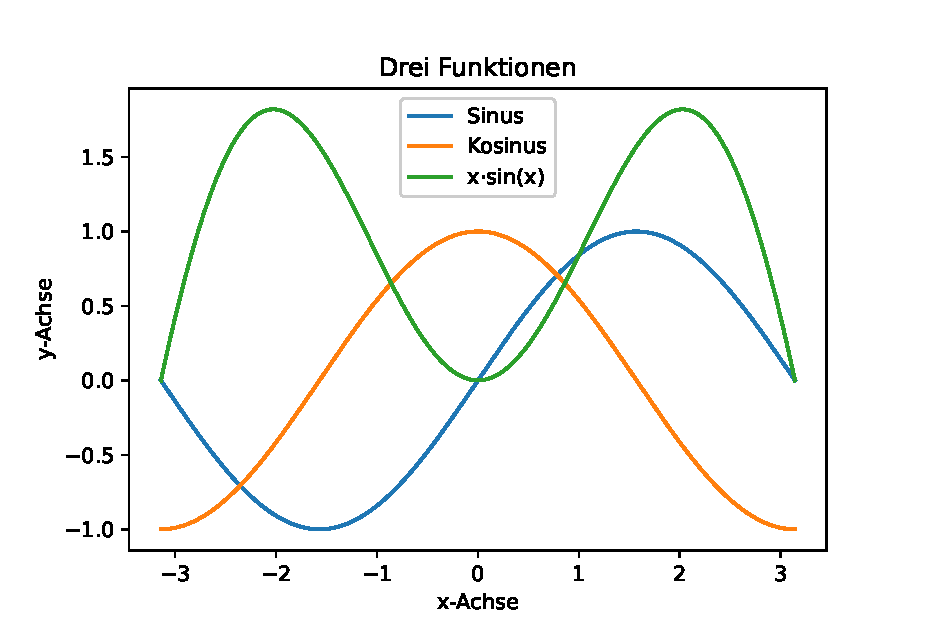
\includegraphics[width=\textwidth]{python/Bild.eps}
    \caption{EPS}
    \label{Abb:EPS}
  \end{subfigure} \\
  \begin{subfigure}[t]{.49\textwidth}
    \centering
    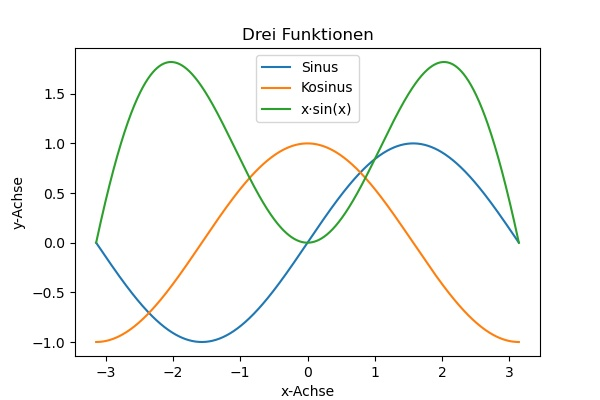
\includegraphics[width=\textwidth]{python/Bild.jpg}
    \caption{JPG}
    \label{Abb:JPG}
  \end{subfigure}
  \begin{subfigure}[t]{.49\textwidth}
    \centering
    \includegraphics[width=\textwidth]{python/Bild.png}
    \caption{PNG}
    \label{Abb:PNG}
  \end{subfigure}  
  \caption{Vergleich verschiedener Bildformate}
  \label{Abb:Bildformate}
\end{figure}
Man sieht, dass man in den Vektorgrafik-Formaten auch die Texte
kopieren kann, bei den anderen Formaten ist das nicht möglich.

\subsection{Sätze und Lemmata}
\label{sec:Saetze_und_Lemmata}

Mathematische Sätze, Beweise, Lemmata und andere Dinge setzt man wie
folgt:
\begin{theorem}
  \label{theo:Wers_glaubt}
  Dieser Satz ist falsch.
\end{theorem}

\begin{proof}
  Es ist ein Satz, das steht doch da. Also muss er zwangsläufig
  korrekt sein.
\end{proof}

Natürlich ist
\hyperref[theo:Wers_glaubt]{Satz~\ref*{theo:Wers_glaubt}} mathematisch
nicht sauber formuliert, also nicht zu lange den Kopf darüber
zerbrechen.

\begin{theorem}
  Der vorangehende Satz ist richtig.
\end{theorem}

\begin{proof}
  Endet ein Beweis in einer Formel, so schiebt man Halmos Box ans Ende
  der Formel, indem man in der Formel \verb|\qedhere| schreibt,
  \[
    a = n. \qedhere
  \]
\end{proof}

\begin{definition}[Primzahl]
  \label{def:Primzahl}
  Eine \emph{Primzahl} $p$ ist eine natürliche Zahl $p\in\N$, welche
  nur zwei verschiedene Teiler hat.
\end{definition}

\begin{lemma}[\v{C}eby\v{s}ev]
  \label{lem:Chebyshev}
  Für alle $n\in\N$ gilt: Im abgeschlossenen Intervall $[n,2n]$ liegt
  immer eine Primzahl $p$.
\end{lemma}

\subsection{Verweise}
\label{sec:Verweise}

Wir haben gesehen, dass man auf Formeln verweisen kann, zum Beispiel
auf
\hyperref[eq:wichtige_Formel]{Gleichung~(\ref*{eq:wichtige_Formel})}
oder auf Abbildungen wie
\hyperref[Abb:EinBeispielbild]{Abbildung~\ref*{Abb:EinBeispielbild}}.
Verweisen kann man auch auf Abschnitte, zum Beispiel auf
\hyperref[sec:Motivation]{Abschnitt~\ref*{sec:Motivation}} oder den
\hyperref[sec:Formeln]{Unterabschnitt zu Formeln}.

Ebenso kann man auf Sätze, Lemmata oder andere mathematische
Umgebungen verweisen, dieses geschieht ohne Klammern um die Nummer,
also zum Beispiel als Verweis auf Lemma~\ref{lem:Chebyshev} oder auf
\hyperref[def:Primzahl]{Definition~\ref*{def:Primzahl}}.

\section{Numerische Ergebnisse}
\label{sec:NumerischeErgebnisse}

Die aufbauend auf den vorangehenden Erläuterungen durchgeführten
numerischen Tests werden in einem Ergebniskapitel vorgestellt. Es
bietet sich das Paket \texttt{listings} an, mit dem man Code diverser
Sprachen direkt einbinden kann. Als Beispiel sei der folgende
Python-Code genannt, den wir in eine \texttt{minipage}-Umgebung
gepackt haben, damit er nicht so viel Platz einnimmt:
\begin{center}
  \begin{minipage}[h]{.7\linewidth}
    \lstinputlisting{python/beispiel.py}
  \end{minipage}
\end{center}

\subsection{Python-Code für Bilder}
\label{sec:Python_Bilder}

Der Python-Code für die Bilder aus
\hyperref[Abb:Bildformate]{Abbildung~\ref*{Abb:Bildformate}} ist
im folgenden Listing enthalten. Dort wird auch gezeigt, wie man die
Größe des Bildes anpasst, so dass die Beschriftungen gut lesbar sind,
sowie gezeigt, wie man überhaupt Achsen beschriftet und einen Titel
und eine Legende hinzufügt:
\medskip
\lstinputlisting{python/bilder.py}

\section{Fazit und Ausblick}
\label{sec:FazitAusblick}

Zu guter Letzt werden die Ergebnisse der Arbeit (positive wie
negative) in einem abschließenden Kapitel kurz, aber verständlich
vorgestellt. Hier ist auch der geeignete Platz für Erweiterungen der
durchgeführten Untersuchungen, wie man sie zum Beispiel in einer
anschließenden Masterarbeit weiter bearbeiten würde.

\printbibliography

\end{document}
